\chapter{Architectuur}
\label{ch:cassandra_architectuur}
% Peer to peer
% Cluster en snitches en partitioners

%Structuur van Cassandra Data Modeling and Analysis
\section{Partitionering}
Een van de belangrijkste zaken bij Cassandra is het horizontaal schalen.
Om dit te kunnen doen moet de data dynamisch gepartitioneerd worden over de nodes van een cluster.
Cassandra krijgt dit voor elkaar door het gebruik van partitioners.
De partitioner wordt ingesteld op cluster niveau.
Deze partitioners maken gebruik van hash functies om te bepalen op welke node de data geplaatst moet worden.
Bij consistente hashing bij Cassandra wordt de output behandeld als een ''ring''.
Elke node in de cluster krijgt een willekeurige waarde toegewezen en deze waarde bepaalt dan de plaats in de ring \citep{lakshman2010cassandra}.


Er zijn drie soorten partitioners in Cassandra:

\begin{enumerate}
	\item \textbf{RandomPartitioner}:
	Dit was de standaard partitioner tot Cassandra 1.2.
	Aan de hand van de MD5 hash van de rijsleutel probeert deze partitioner de data evenwichtig over alle nodes te verspreiden.
	Omdat de MD5 Hash functie vrij traag is, werd er een andere partitioner als standaard aangesteld.
	
	\item \textbf{Murmur3Partitioner}:
	Sinds Cassandra 1.2 is dit de standaard partitioner van deze databank.
	Deze partitioner maakt gebruik van de MurmurHash functie, waardoor de hash een 64-bit hashwaarde van de rijsleutel wordt.
	
	\item \textbf{ByteOrderedPartitioner}:
	Zoals de naam doet vermoeden wordt deze partitioner gebruikt voor geordende partitionering.
	Deze partitioner ordent de rijen volgens de bytes van de rijsleutel.
	De tokens worden berekend aan de hand van de hexadecimale representatie van de leidende tekens van de rijsleutel.
	Op deze manier kan men, net zoals men met een cursor in een SQL omgeving zou doen, de tabel geordend overlopen, gesorteerd op primaire sleutel.
	
\end{enumerate}

\subsection{Problemen met de ByteOrderedPartitioner}
De ByteOrderedPartitioner blijkt een oplossing te bieden om tabellen te verkrijgen die gesorteerd zijn op de primaire sleutel.
Ondanks dit feit zijn er toch een aantal problemen met deze partitioner:

\begin{itemize}
	\item Sequentiële writes kunnen voor ''hot spots'' zorgen.
	Als een aantal rijen ongeveer gelijktijdig toegevoegd of geüpdatet worden, dan worden deze quasi zeker op dezelfde node weggeschreven.
	Dit vormt bijvoorbeeld een groot probleem bij tijdreeksen \citep{kan2014cassandra}.
	
	\item Met de ByteOrderedPartitioner is het zeer moeilijk om een gebalanceerde cluster te krijgen.
	De enige manier waarop dit verkregen kan worden is om dit manueel te doen.
	Als men dit echter niet doet is de kans vrij groot dat de data op slechts enkele nodes van de cluster opgeslagen wordt.
	Als men dan nog eens verschillende types voor de primaire sleutels definieert is het zo goed als onmogelijk om een gebalanceerde cluster te krijgen
	\citep{Bauer2013CaseAgainstByteOrder}.
\end{itemize}

\section{Replicatie}
\label{sec_replication}
Om de hoge beschikbaarheid te verkrijgen maakt Cassandra gebruik van data replicatie.
Door de replicatie wordt de kans op een ''Single point of Failure'' enorm beperkt.
Cassandra biedt een methode aan om de replicatie factor te blijven behouden zelfs indien bepaalde nodes uitgevallen zouden zijn.
Deze replicatie factor wordt ingesteld op keyspace niveau.
De replicatie factor bepaalt hoeveel replica's van de data bijgehouden worden.
Op basis van de partitioner en de replicatie strategie wordt  bepaald waar de replica's opgeslagen worden.
Om deze replicatie in goede banen te leiden zijn er een aantal strategieën uitgewerkt \citep{kan2014cassandra}.

\subsection{Replicatie strategieën}
% p63
De replicatie strategie bepaalt waar de data precies op de cluster geplaatst wordt.
Hierbij zijn er twee strategieën:

\subsubsection{SimpleStrategy}
Deze SimpleStrategy wordt meestal gebruikt als er maar één datacenter aanwezig is.
Wanneer men over meerdere datacenters beschikt is het beter om naar de andere strategie te kijken.
Wanneer de standaard partitioner, de Murmer3Partitioner, gebruikt wordt gaat de partitioner de locatie bepalen aan de hand van de hash van de primaire sleutel.
De replica's van de data worden geplaatst op de volgende nodes in de ring met de richting van de klok mee.
	
Op figuur \ref{fig:simple_strategy} wordt een voorbeeld gegeven waarbij de replicatie factor 3 is.
De zwarte namen zijn de originele data en de grijze de replica's.
	
\begin{figure}[H]
	\centering
	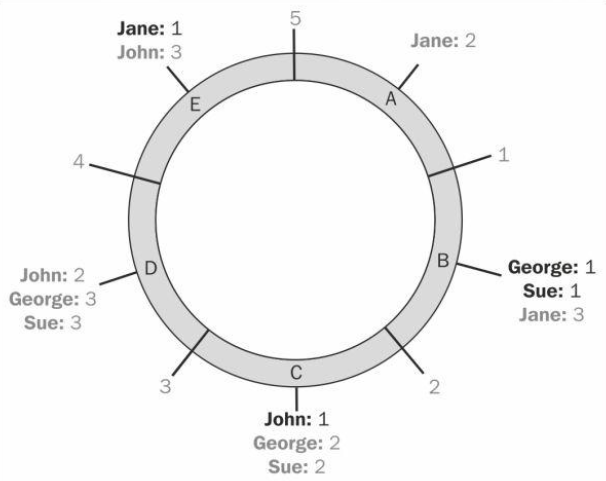
\includegraphics[width=0.75\textwidth]{img/4_architectuur/SimpleStrategy}
	\caption{Illustratie SimpleStrategy \citep{strickland2014availability}}
	\label{fig:simple_strategy}
\end{figure}
	
	
\subsubsection{NetworkTopologyStrategy}
Op productieclusters wordt vaak de NetworkTopologyStragegy toegepast.
Hierbij gaat men ervan uit dat een productiecluster uit meerdere datacenters bestaat of in de toekomst meerdere datacenters zal bevatten.

Het grote voordeel van deze strategie is dat er rack awareness is en dat de snitches ingesteld kunnen worden.
Rack awareness zorgt ervoor dat de replica's op verschillende racks worden opgeslagen.
Dit is echter niet mogelijk bij SimpleStrategy.
Ook kan men door het gebruik van deze strategie voor ieder datacenter een andere replicatie factor instellen.

\section{Snitches}
Een snitch is verantwoordelijk om de data snel en efficiënt op te halen binnen de cluster.
Een andere verantwoordelijkheid van een snitch is om mee te helpen bepalen waar de replica's fysiek opgeslagen worden.
Er zijn acht soorten snitches beschikbaar op Cassandra \citep{strickland2014availability}.

\begin{enumerate}
	\item \textbf{SimpleSnitch}:
	Deze snitch gaat altijd samen met SimpleStrategy en is speciaal ontworpen voor eenvoudige datacenters.
	
	\item \textbf{RackInferringSnitch}:
	Deze snitch probeert de netwerk topologie van de cluster te achterhalen.
	Het gebruik van deze snitch wordt echter sterk afgeraden.
	Het probleem is hier dat ervan uitgegaan wordt dat het ip-adres de structuur van het datacenters en de racks reflecteert.
	
	\item \textbf{PropertyFileSnitch}:
	Met deze snitch kan de administrator zelf instellen welke nodes tot welke rack en datacenter behoren.
	Als men deze snitch gebruikt moet men dus de ganse topologie uitschrijven. 
	Iedere node moet ook precies op dezelfde manier geconfigureerd worden.
	Dit alles heeft veel overhead als er nodes toegevoegd of verwijderd moeten worden.
	
	\item \textbf{GossipingPropertyFileSnitch}:
	De GossipingPropertyFileSnitch lijkt zeer sterk op de PropertyFileSnitch.
	Het grote verschil is dat men per rack en datacenter maar één node hoeft te configureren.
	Daarna verspreidt de snitch de configuratie van deze node naar alle andere nodes.
	
	\item \textbf{CloudStackSnitch}:
	Deze snitch de datacenters en racks op volgens CloudStack's land, locatie en beschikbaarheid zones.
	
	\item \textbf{GoogleCloudSnitch}:
	De GoogleCloudSnitch is speciaal gemaakt voor Cassandra binnen Google Cloud.
	Hierbij zet deze snitch de locatie als datacenter en de beschikbaarheidszone als rack.
	
	\item \textbf{EC2Snitch}:
	Deze snitch is zeer gelijkaardig aan de GoogleCloudSnitch.
	Net zoals bij de vorige snitch wordt de regio als datacenter ingesteld en de beschikbaarheidszone als rack.
	
	\item \textbf{EC2MultiRegionSnitch}:
	Deze snitch werkt op identiek dezelfde manier als de EC2Snitch.
	Het enige verschil hier is dat deze snitch publieke ip-adressen toestaat voor communicatie tussen verschillende datacenters.
	
\end{enumerate}

Voor productieomgevingen is de GossipingPropertyFileSnitch meestal de beste keuze wanneer er met fysieke datacenters wordt gewerkt.
Als men in de cloud werkt kiest men best voor de bijhorende snitch.

\section{Seed node}
Sommige nodes in de Cassandra cluster zijn seed nodes.
De configuratie van deze seed node wordt gebruikt bij het bootstrappingproces wanneer er nieuwe nodes aan de cluster toegevoegd worden.
De nieuwe node zal eerst communiceren met de seed node om zo informatie over de andere nodes in de cluster te bekomen.
Hoewel er technisch gezien maar één seed node nodig is per cluster, is het toch sterk aangeraden om meerdere seed nodes per datacenter beschikbaar te stellen \citep{kan2014cassandra}.